\chapter{Relevant literature}
\label{ch:literature}

In this chapter, a summary of the most important aspects of \citet{deBoer2000} is given.
We also discuss some literature on network structures in ABMs to further defend why we think our extension is a useful one.

%------------------------------------

\section{Summary of de Boer (2000)}
\label{sec:literature_db2000}

It was seen from previous work, such as that by \citet{landl}, that functional properties give rise to human-like vowel systems.
Such findings are often found through direct optimisation, in the case of \citep{landl} this is by doing a minimisation on the potential energy to find that optimising for acoustic difference gives rise to realistic vowel systems.
However, whilst such findings are great, they give rise to another question, \textit{how} does this optimisation take place.
This \textit{how} question is one that \citep{deBoer2000} tries to understand by studying an ABM playing imitation games.
This paper of \citet{deBoer2000} is inspired by his PhD thesis, which is longer and more detailed \citep{deBoerFull}.
If the ABM, which makes use of simple self-organised agents, gives rise to human-like vowel systems, it \textit{could} be possible that self-organisation played an important role in the evolution of speech.
This could part is important, as ABMs can't directly prove a hypothesis.

The ABM described by \citet{deBoer2000} consists of agents who play imitation games.
These imitation games consist of two randomly picked agents where one is the \textit{speaker} and the other is the \textit{imitator}.
The speaker says a random sound from his \textit{sound repetoire}.
The imitator replies with one of his known sounds that lies closest to the \textit{perceived} one.
The speaker then communicates a \textit{non-verbal} signal to either confirm or reject the imitation to be correct.
A correct imitation is one where the perceived sound is closest to the initially produced sound for the speaker.
The imitator uses this information to update his sound repertoire.
The sound repertoires of agents are non-fixed and initially empty.
From this description it becomes clear an agent should have three important skills: a sound \textit{production}, \textit{perception}, and \textit{storing} mechanism.
Besides this, the agent should also be able to \textit{learn} from the non-verbal signals.
Chapter \ref{ch:reimplementing} re-implements this ABM, where it is described in more detail how these different components work and some of the \textit{ad hoc} decisions made by \citet{deBoer2000} to make it work.

Chapter \ref{ch:reimplementing} goes into more detail on the metrics used to evaluate the findings of this ABM.
In that chapter, the found evaluation metrics are also replicated.
From these found results, \citet{deBoer2000} concludes that self-organization can explain properties found in human vowel systems.
He states that one should not study a vowel system by its individual vowels (as done by \cite{chomsky}) or as a whole \citep{landl} but rather concerning the population it is used in.
This work by \citet{deBoer2000} remains one of his most cited works and has proven to be influential in the field.
Because of this, we found it fit to re-implement it so that newcomers can get a grasp on experiments in the field and to further defend the findings by \citet{deBoer2000}.







%------------------------------------

\section{Importance of network structure for emergence}
\label{sec:literature_emergence}

The extension to the above discussed ABM provided with this report is one on the network structure used.
As discussed, the pair of agents to play an imitation game each iteration are chosen at random in the implementation of \citet{deBoer2000}.
Given enough iterations, this will evolve from a random network to a fully connected network.
This contradicts with human networks where a certain hierarchy exists and not every person will adopt his speech to another person.
For example, a professor in the English language would not adopt his sound repertoire to that of a newborn.
More importantly, the results of ABMs have been shown to depend heavily on the underlying communication network used, whether they are used in linguistic applications or not \citep{network1, network2, network3}.

To model human communities, scale-free networks are often used.
Scale-free networks are networks where the degree distribution of nodes follows a power law.
A preferential attachment like property in human psychology is often given as a reason that these networks are well representative of a human social network \citet{scalefreegood}.
However, it is often debated whether such scale-free networks appear as often in nature as it is claimed to by some \citep{scalefreebad}.

Another commonly used network is a \textit{small-world} network.
An overview of these three network structures is given in Figure \ref{fig:network_structures}.
Many other network structures exist as it is an important topic of graph theory.
We believe a network that lies between small-world and scale-free networks is a good fit to represent early human communities.
Hence, such a directed and weighted network is presented in chapter \ref{ch:extension}.


\begin{figure}[H]
    \centering
    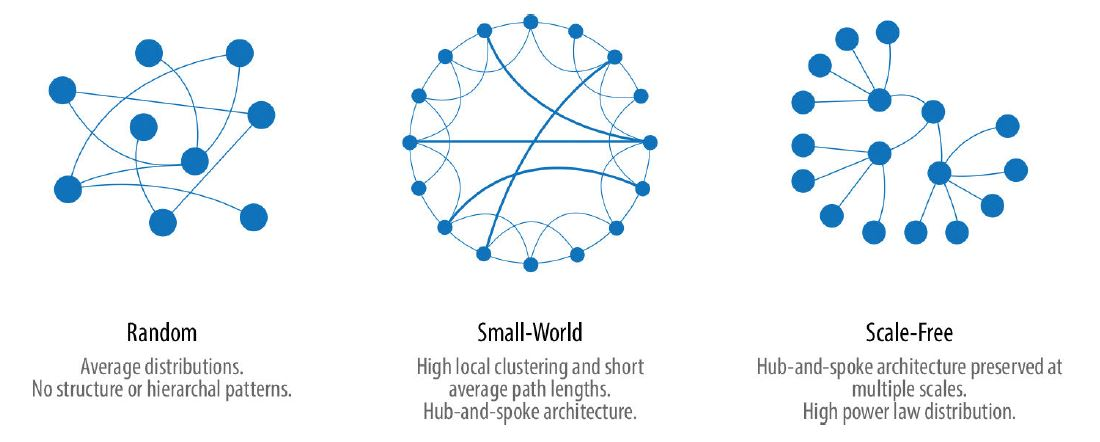
\includegraphics[width=\linewidth]{images/literature/network_structures.jpeg}
    \captionsetup{width=0.9\linewidth}
    \captionsetup{justification=centering}
    \caption{Random, small-world and scale-free networks. Figure by \citet{graphsfigure}.}
    \label{fig:network_structures}
\end{figure}

